\documentclass{article}

\usepackage[preprint]{neurips_2024}

\usepackage[utf8]{inputenc}
\usepackage[T1]{fontenc}
\usepackage{hyperref}
\usepackage{url}
\usepackage{booktabs}
\usepackage{amsfonts}
\usepackage{amsmath}
\usepackage{amssymb}
\usepackage{nicefrac}
\usepackage{microtype}
\usepackage{xcolor}
\usepackage{algorithm}
\usepackage{algpseudocode}
\usepackage{graphicx}
\usepackage{multirow}
\usepackage{makecell}
\usepackage{natbib}
\usepackage{tablefootnote}

\title{SGSR-2: Measured-Cost Pareto Allocation of Bit-Width and\\
Group-Size for On-Device LLM Quantization}

\author{
  Matthias Raviotta \\
  Independent Research \\
  \texttt{raviottamatthias@gmail.com}
}

\begin{document}

\maketitle

\begin{abstract}
We present \textbf{SGSR-2}, a post-training quantization method that jointly
allocates per-block bit-width and group-size for large language models using
\emph{measured} quantization cost rather than heuristic proxies. For each
transformer block and each configuration $(b, k)$ with bits
$b\in\{3,4,5,6\}$ and group size $k\in\{32,64,128\}$, we measure the KL
divergence of output logits under reversible fake-quantization of that block
alone. A validated additivity assumption then reduces budget-constrained
allocation to an exact per-block Lagrangian rule, yielding the complete
3--5~bit/w Pareto frontier from a single overnight profiling run on consumer
hardware (Apple M1~Pro, 32~GB). Under a unified accounting protocol
(on-disk size over total parameters, full Wikitext-2 sliding-window
perplexity), SGSR-2 strictly dominates uniform MLX quantization on both
TinyLlama-1.1B and Qwen2.5-7B---e.g.\ $+18.7\%$ PPL at 3.62~bit/w versus
$+36.0\%$ at 3.93~bit/w for the best uniform setting on Qwen---and matches or
outperforms the hand-tuned llama.cpp K-quants frontier at
$\geq\!4.4$~bit/w, while losing to \texttt{Q3\_K\_M} below 4~bit/w, a gap we
attribute to storage-format richness rather than allocation quality. We also
report a negative result that corrects our earlier work (SGSR~v1): under
controlled baselines, Shannon-entropy sensitivity ranking is statistically
indistinguishable from random ranking on both models, and the previously
reported gains are explained by a SmoothQuant confound. All code, cost
tables, and results are released; the method is gradient-free and runs
entirely on-device.
\end{abstract}

\vspace{0.5em}
\noindent\textit{This paper supersedes SGSR~v1 (Zenodo, July 2026). Section~\ref{sec:negative}
reports the controlled experiments that overturned v1's central claim.}

\section{Introduction}

Deploying large language models on consumer hardware requires aggressive
weight compression. Post-training quantization (PTQ) is the dominant
approach \citep{gptq, llmint8}. Two design axes govern the quality/size
trade-off of group-wise PTQ: the \emph{bit-width} of each weight and the
\emph{group size} over which quantization scales are shared. Smaller groups
reduce quantization error but pay metadata overhead; in MLX's affine format
each group of $k$ weights carries a bf16 scale and bias, i.e.\
$32/k$ extra bits per weight. In practice both axes are set uniformly
across all layers.

Transformer blocks, however, differ widely in their sensitivity to
quantization error. Our earlier work (SGSR~v1) attempted to exploit this by
ranking layers with Shannon entropy and redistributing group sizes by rank.
When we later added the controls that v1 lacked---the same SmoothQuant
pre-processing on the uniform baseline, random and inverted rankings, and a
uniform fine-group baseline---the entropy signal vanished entirely
(Section~\ref{sec:negative}). The lesson is general: \emph{heuristic proxies
for sensitivity must be validated against randomized controls before they
are used to allocate anything.}

SGSR-2 replaces the proxy with measurement. We fake-quantize one block at a
time, measure the resulting KL divergence on the output logits over a fixed
calibration set, and record a cost table $e_l(c)$ for every block $l$ and
configuration $c=(b,k)$. If total degradation is approximately additive
across blocks---an assumption we test explicitly and quantify---then
minimizing predicted cost under an effective-bits budget decomposes into an
exact per-block rule $c_l(\lambda) = \arg\min_c\, e_l(c) + \lambda\,
p_l\,\beta(c)$, where $p_l$ is the block's parameter count and $\beta(c)$
its effective bits per weight. Sweeping the multiplier $\lambda$ traces the
entire Pareto frontier at negligible cost: one profiling run, every budget.

Our contributions are:
\begin{enumerate}
  \item \textbf{A measured, gradient-free cost model} for joint
    (bit-width, group-size) allocation: per-block KL cost tables computed
    with reversible fake-quantization and a streaming top-$K$ logit
    approximation, entirely on-device.
  \item \textbf{An explicit additivity gate}: we validate that predicted
    (summed) costs track measured full-plan costs (ratio 0.74--1.11, rank
    order preserved) before trusting the allocator.
  \item \textbf{An exact Lagrangian allocator} over the joint configuration
    space, producing the full 3--5~bit/w frontier from one cost table.
  \item \textbf{A unified evaluation protocol}: all methods---ours, uniform
    MLX, and llama.cpp K-quants---are compared by on-disk size over total
    parameters, with full-test-set sliding-window perplexity and bootstrap
    confidence intervals. This corrects inconsistent accounting in v1.
  \item \textbf{A documented negative result}: entropy ranking is
    indistinguishable from random ranking on both models once the
    SmoothQuant confound is removed.
\end{enumerate}

\section{Method}

\subsection{Measured per-block cost tables}
\label{sec:profiler}

Let a model have blocks $l = 1,\dots,L$ (transformer decoder layers; all
weight matrices within a block share one configuration). The configuration
space is $\mathcal{C} = \{3,4,5,6\} \times \{32,64,128\}$ (12
configurations); 2-bit is excluded due to catastrophic degradation and
8-bit is never optimal below a 5~bit/w average budget.

\paragraph{Reversible fake-quantization.}
For block $l$ and configuration $c$, we replace every 2-D weight $W$ in the
block with $\mathrm{dequant}(\mathrm{quant}(W; c))$, keeping computation in
BF16. The original tensors are retained and restored bit-exactly after
measurement (guaranteed also on exceptions). Weight selection is fixed
across all configurations (alignment to the largest group size), so every
entry of the cost table measures the identical weight set---costs are
comparable across configurations by construction.

\paragraph{Streaming KL cost.}
Storing full baseline logits for the calibration set is infeasible
(sequence length $\times$ vocabulary $\approx$ 150k). We snapshot, per
token, the top-64 baseline log-probabilities plus a residual tail mass, and
compute
\begin{equation}
  e_l(c) \;=\; \mathbb{E}_{\text{tokens}}\Bigl[\,\sum_{i \in \text{top-64}}
  p_i \log\frac{p_i}{q_i} \;+\; m_p \log\frac{m_p}{m_q}\Bigr] \;\geq\; 0,
\end{equation}
where $p$ is the baseline distribution, $q$ the distribution under
fake-quantization of block $l$, and $m$ the respective tail masses. The
calibration set is fixed and reproducible: 32 sequences of 512 tokens from
Wikitext-2 train, seed 42. Profiling all $L \times |\mathcal{C}|$ entries
takes one overnight run for a 7B model on M1~Pro; the table is cached and
checkpointed per block, so interrupted runs resume.

\subsection{Additivity gate}
\label{sec:gate}

The allocator assumes total cost is approximately the sum of per-block
costs. Before using it, we test this: for three plans spanning the budget
range we apply the \emph{full plan} in fake-quantization and compare the
measured KL against the predicted sum (Table~\ref{tab:gate}). Acceptance
requires preserved rank order and prediction/measurement ratios within
$[0.5, 1.5]$. The gate passed on first evaluation; had it failed, the
protocol prescribes conditional re-measurement of the highest-cost blocks.

\begin{table}[t]
\centering
\caption{Additivity gate on TinyLlama-1.1B. Predicted $=\sum_l e_l(c_l)$;
measured $=$ KL of the full plan applied jointly. Rank order across the
three plans is preserved.}
\label{tab:gate}
\begin{tabular}{cccc}
\toprule
\textbf{Plan (eff.\ bit/w)} & \textbf{Predicted} & \textbf{Measured} & \textbf{Ratio} \\
\midrule
3.25 & 0.2478 & 0.3351 & 0.74 \\
3.81 & 0.1203 & 0.1389 & 0.87 \\
4.61 & 0.0419 & 0.0378 & 1.11 \\
\bottomrule
\end{tabular}
\end{table}

\subsection{Exact Lagrangian allocation}
\label{sec:allocator}

Define effective bits $\beta(b,k) = b + 32/k$ (bf16 scale and bias per
group) and let $p_l$ be block $l$'s parameter count. The budget-constrained
problem
\begin{equation}
  \min_{\{c_l\}} \sum_l e_l(c_l)
  \quad\text{s.t.}\quad
  \frac{\sum_l p_l\, \beta(c_l)}{\sum_l p_l} \;\leq\; B
\end{equation}
decomposes, under additivity, into the per-block rule
\begin{equation}
  c_l(\lambda) \;=\; \arg\min_{c \in \mathcal{C}} \; e_l(c) + \lambda\, p_l\, \beta(c).
\end{equation}
Sweeping $\lambda$ over an adaptive range (anchored to each block's
$\Delta e / (p_l\, \Delta\beta)$ turning points, with $\lambda{=}0$ included
to guarantee the max-bits extreme) traces the frontier; deduplication by
assignment yields the discrete Pareto set. For any requested budget we
select the feasible point of minimum predicted cost. Fallback bits for
modules outside the per-block plan (embeddings) track the parameter-weighted
mean of the assigned block bits, keeping comparisons with uniform baselines
fair. The allocator is pure post-processing: new budgets cost milliseconds
once the table exists.

\section{Experimental setup}
\label{sec:setup}

\paragraph{Models and hardware.}
TinyLlama-1.1B-Chat-v1.0 \citep{tinyllama} and Qwen2.5-7B-Instruct
\citep{qwen25}; Apple M1~Pro, 32~GB unified memory, MLX \citep{mlx} 0.31,
BF16. No external accelerator at any stage.

\paragraph{Evaluation protocol.}
Perplexity on the \emph{full} Wikitext-2 test set \citep{wikitext},
sliding window 2048 with stride 512 (each token scored exactly once with at
least 1536 tokens of context), 95\% bootstrap confidence intervals over
per-token negative log-likelihoods. SmoothQuant \citep{smoothquant}
($\alpha{=}0.5$) is applied to \emph{all} MLX-quantized variants including
uniform baselines, removing the confound of v1.

\paragraph{Unified bits accounting.}
For every method, bits per weight $=$ on-disk model size $\times 8$ divided
by \emph{total} parameter count. This penalizes all metadata (scales,
biases, embeddings) identically across methods and matches how K-quants
sizes are conventionally reported. We flag that v1 mixed two accounting
conventions in one table; all numbers here use the unified rule.

\paragraph{Baselines.}
(i)~Uniform MLX affine quantization at $(b,k) \in \{3,4,5\} \times
\{32,64,128\}$ with SmoothQuant; (ii)~llama.cpp K-quants
\citep{llamacpp} \texttt{Q3\_K\_M}, \texttt{Q4\_K\_M}, \texttt{Q5\_K\_M},
evaluated with \texttt{llama-perplexity} (context 2048) on the byte-identical
test text, reported as $\Delta$PPL relative to the f16 GGUF baseline of the
same runtime, which controls for protocol differences between runtimes.

\section{Results}
\label{sec:results}

\begin{table}[t]
\centering
\caption{Main results under unified accounting (bit/w $=$ disk size
$\times$ 8 / total parameters). $\Delta$PPL\% relative to each runtime's own
full-precision baseline; full Wikitext-2 test, sliding window. Uniform
rows include SmoothQuant. The Qwen uniform sweep at 4--5 bits was
truncated by an interrupted run (Section~\ref{sec:limits}); measured points
only.}
\label{tab:main}
\setlength{\tabcolsep}{5pt}
\begin{tabular}{llcc@{\hspace{1.5em}}cc}
\toprule
& & \multicolumn{2}{c}{\textbf{TinyLlama 1.1B}} &
    \multicolumn{2}{c}{\textbf{Qwen2.5-7B}} \\
\cmidrule(lr){3-4}\cmidrule(l){5-6}
\textbf{Family} & \textbf{Setting} & bit/w & $\Delta$PPL\% & bit/w & $\Delta$PPL\% \\
\midrule
\multirow{4}{*}{SGSR-2 (ours)}
 & budget 3.25 & 3.28 & +45.4 & 3.29 & +69.6 \\
 & budget 3.5  & 3.49 & +27.0 & 3.40 & +25.5 \\
 & budget 4.0  & 3.83 & \textbf{+14.3} & 3.62 & \textbf{+18.7} \\
 & budget 4.5  & 4.44 & \textbf{+4.65} & 4.55 & \textbf{+3.97} \\
\midrule
\multirow{7}{*}{Uniform MLX + SQ}
 & 3-bit, $k{=}128$ & 3.28 & +45.4 & --- & --- \\
 & 3-bit, $k{=}64$  & 3.50 & +30.9 & 3.50 & +48.3 \\
 & 3-bit, $k{=}32$  & 3.94 & +23.1 & 3.93 & +36.0 \\
 & 4-bit, $k{=}128$ & 4.28 & +6.45 & --- & --- \\
 & 4-bit, $k{=}64$  & 4.50 & +4.75 & --- & --- \\
 & 4-bit, $k{=}32$  & 4.94 & +3.42 & --- & --- \\
 & 5-bit, $k{=}64$  & 5.50 & +0.94 & --- & --- \\
\midrule
\multirow{3}{*}{llama.cpp K-quants}
 & \texttt{Q3\_K\_M} & 3.99 & +7.47 & 4.00 & +7.79 \\
 & \texttt{Q4\_K\_M} & 4.86 & +2.97 & 4.92 & +1.98 \\
 & \texttt{Q5\_K\_M} & 5.69 & +0.80 & 5.72 & +0.66 \\
\bottomrule
\end{tabular}
\end{table}

\begin{figure}[t]
  \centering
  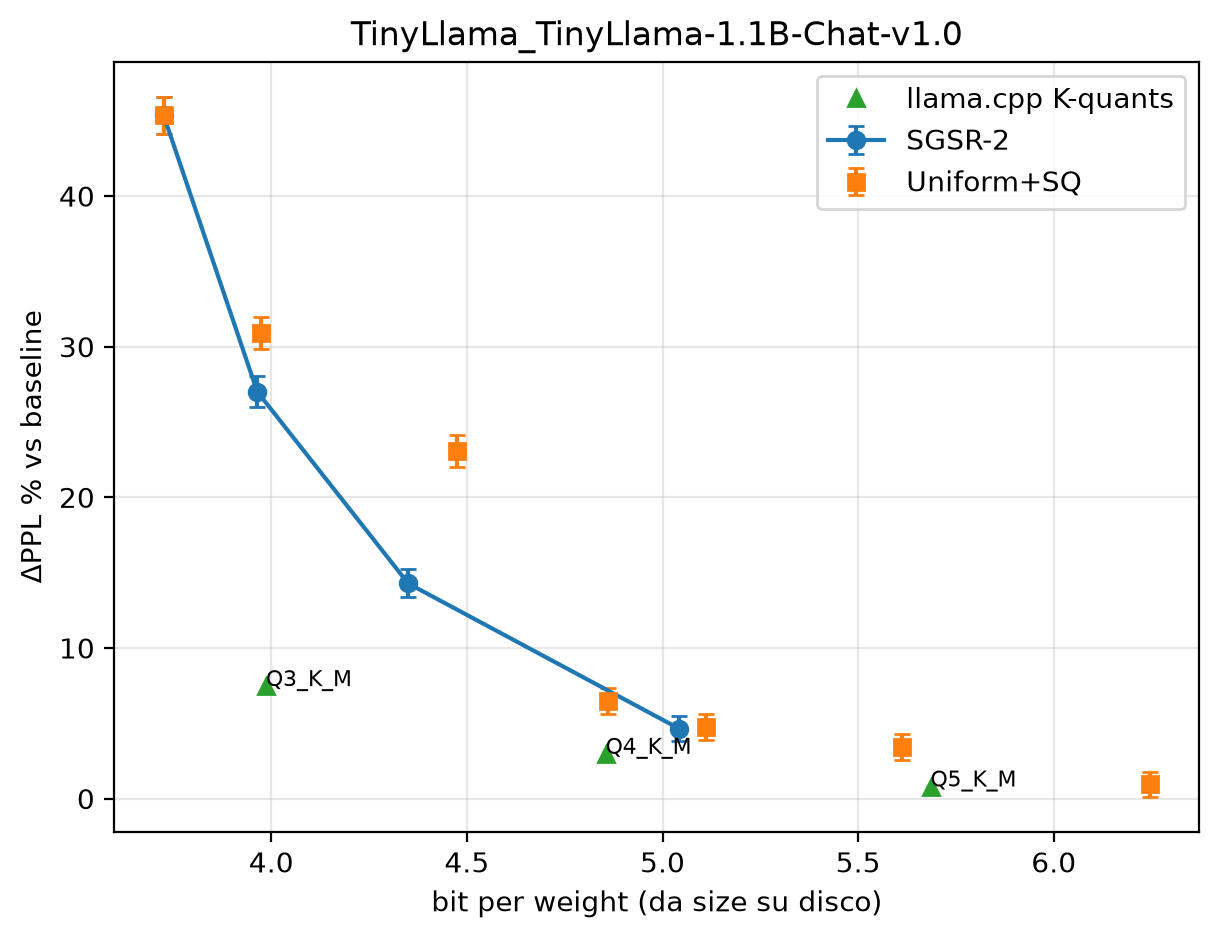
\includegraphics[width=0.49\linewidth]{figures/pareto_TinyLlama_TinyLlama-1.1B-Chat-v1.0.png}
  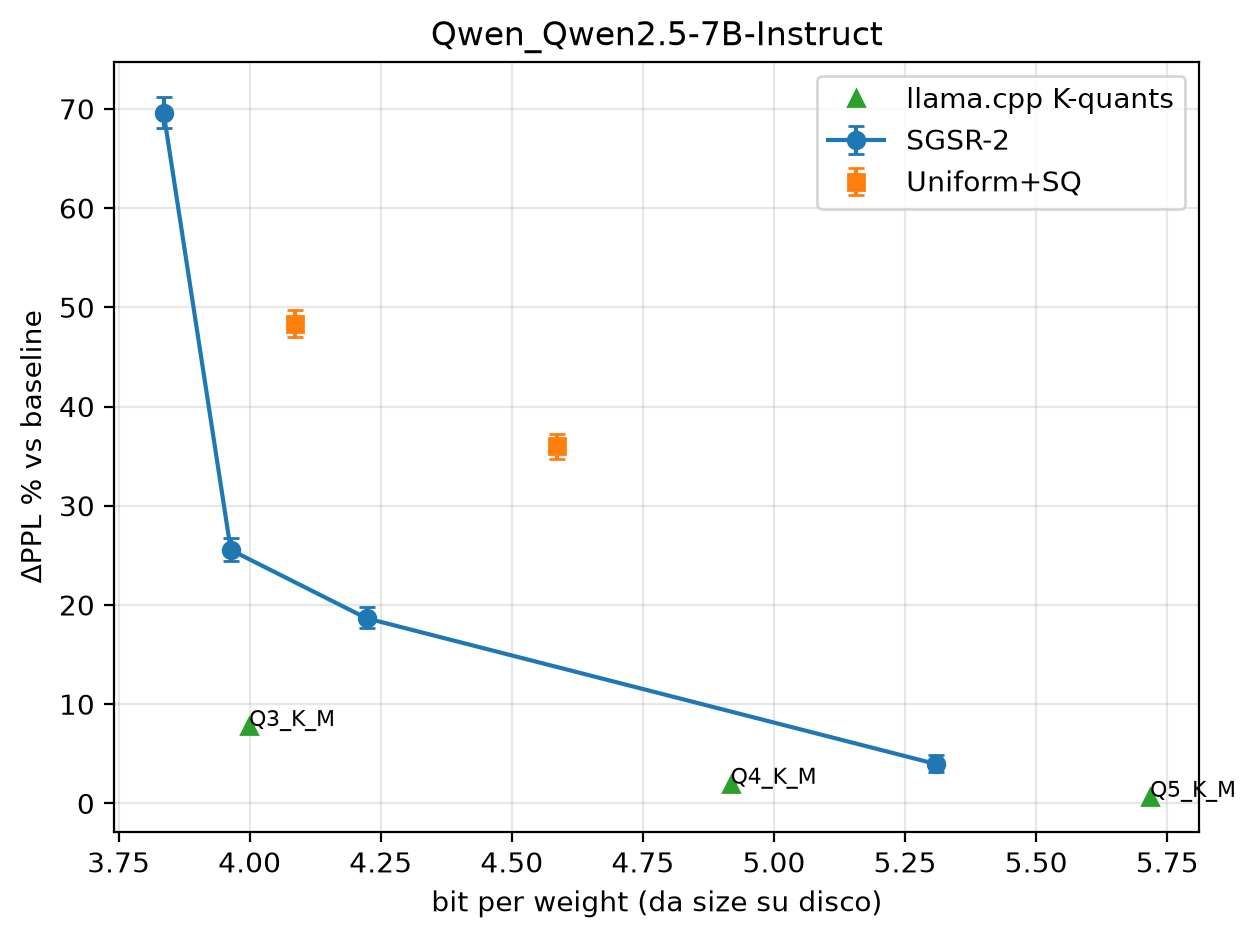
\includegraphics[width=0.49\linewidth]{figures/pareto_Qwen_Qwen2.5-7B-Instruct.png}
  \caption{PPL-vs-bits frontiers for TinyLlama-1.1B (left) and Qwen2.5-7B
  (right). Error bars are 95\% bootstrap CIs on per-token NLLs.}
  \label{fig:pareto}
\end{figure}

\paragraph{SGSR-2 versus uniform MLX quantization.}
SGSR-2 strictly dominates the uniform frontier in the 3.4--4.5~bit/w
region on both models. On Qwen, SGSR-2 reaches $+18.7\%$ at 3.62~bit/w
where the best measured uniform setting yields $+36.0\%$ at
\emph{more} bits (3.93); at 3.40~bit/w SGSR-2 roughly halves the uniform
degradation ($+25.5\%$ vs.\ $+48.3\%$ at 3.50). On TinyLlama the pattern is
identical ($+14.3\%$ at 3.83 vs.\ $+23.1\%$ at 3.94). At the budget floor
the allocator correctly degenerates to the uniform minimum configuration
(identical numbers at 3.28~bit/w), and above ${\sim}4.5$~bit/w the two
families converge as all configurations become quality-saturated.

\paragraph{SGSR-2 versus K-quants.}
The comparison splits cleanly at ${\sim}4.4$~bit/w. Above it, SGSR-2 sits
on or below the interpolated K-quants frontier on both models: on Qwen,
$+3.97\%$ at 4.55~bit/w against an interpolated ${\approx}+4.3\%$; on
TinyLlama, $+4.65\%$ at 4.44 against ${\approx}+5.2\%$. Below 4~bit/w,
\texttt{Q3\_K\_M} is clearly stronger ($+7.8\%$ at 4.00 vs.\ our $+18.7\%$
at 3.62 on Qwen). We attribute this gap to the storage format rather than
the allocation: K-quants use super-blocks with 6-bit sub-scales and
per-sub-block minima, a substantially richer low-bit representation than
MLX's affine format (bf16 scale/bias per group), which is the space SGSR-2
allocates over. Where format richness is not the bottleneck
($\geq$4.4~bit/w), measured allocation matches or beats hand-tuned
heuristics; where it is, no allocation policy over the poorer format
closes the gap. Extending MLX with a super-block format---and letting the
same cost-table machinery allocate over it---is the natural next step, and
MLX's recently added \texttt{mxfp4} mode (shared 8-bit scale per 32-group)
is a first candidate.

\section{Negative result: entropy ranking is indistinguishable from random}
\label{sec:negative}

SGSR~v1 reported that entropy-ranked group-size redistribution improved on
uniform 4-bit quantization ($+3.28\%$ vs.\ $+4.34\%$ on TinyLlama). Two
controls, absent in v1, overturn this conclusion
(Table~\ref{tab:negative}): (i)~applying SmoothQuant to the uniform
baseline---v1 applied it only to the treatment arm---already brings uniform
to $+3.00\%$, \emph{ahead} of v1's SGSR at equal effective bits; (ii)~the
entropy ranking performs within the spread of random rankings on both
models, and an \emph{inverted} entropy ranking performs the same as the
correct one. The v1 improvement is therefore explained by the SmoothQuant
confound, and the entropy proxy carries no allocation signal at this
granularity. We report this correction explicitly so that others do not
build on the retracted claim.

\begin{table}[t]
\centering
\caption{Controlled re-evaluation of SGSR~v1's entropy ranking (all
variants 4-bit with SmoothQuant; v1's 100-sample evaluation protocol,
retained here for comparability with v1; effective bits within
$\pm 0.01$ across rankings). Entropy is inside the random spread on both
models; inverted ranking matches the correct one.}
\label{tab:negative}
\begin{tabular}{lcc}
\toprule
\textbf{Ranking / baseline} & \textbf{TinyLlama} $\Delta$PPL\% & \textbf{Qwen2.5-7B} $\Delta$PPL\% \\
\midrule
Uniform $k{=}64$ + SQ (control) & \textbf{+3.00} & \textbf{+10.47} \\
Entropy tiers (v1)              & +3.28 & +10.88 \\
Random tiers (3 seeds / 1 seed) & +3.26 -- +3.93 & +10.84 \\
Inverted entropy tiers          & +3.34 & +11.00 \\
\bottomrule
\end{tabular}
\end{table}

\section{Related work}

\paragraph{Post-training quantization.}
GPTQ \citep{gptq} minimizes layer-wise reconstruction error with
approximate second-order information; AWQ \citep{awq} protects salient
channels identified by activation magnitudes; SpQR \citep{spqr} isolates
sparse outliers at higher precision; SmoothQuant \citep{smoothquant}
rescales activation difficulty into weights and is our pre-processing step.

\paragraph{Sensitivity-guided mixed precision.}
ZeroQ \citep{zeroq} measures per-layer sensitivity via KL divergence and
selects bit-widths along a Pareto frontier; HAWQ-v3 \citep{hawqv3} solves
bit allocation as integer programming under Hessian sensitivity. SGSR-2
differs in three respects: the allocation space is the joint
(bit-width, group-size) grid with metadata overhead inside the budget
constraint; the cost signal is measured output-KL under fake-quantization
of the actual target format (no Hessian or gradient); and the additivity
assumption underlying the decomposed solver is explicitly tested rather
than assumed. EWQ \citep{ewq} uses entropy for bit-width selection; our
Section~\ref{sec:negative} suggests caution with entropy proxies absent
randomized controls.

\paragraph{Deployment-grade formats.}
llama.cpp's K-quants \citep{llamacpp} are hand-designed super-block
formats with empirically chosen per-tensor mixes; they are the de-facto
consumer standard and our external baseline. Our results position measured
allocation as complementary to format design: allocation wins where formats
are comparable, formats win below 4~bit/w.

\section{Limitations}
\label{sec:limits}

(i)~The uniform Qwen sweep at 4--5~bit/w is incomplete (an interrupted run;
the measured 3-bit points suffice for the low-budget comparison but the
4-bit uniform column on Qwen is absent). (ii)~The K-quants frontier below
4~bit/w (\texttt{Q2\_K}, \texttt{Q3\_K\_S}) was not sampled. (iii)~MLX and
llama.cpp perplexity protocols differ in windowing; we mitigate by
reporting deltas against each runtime's own full-precision baseline.
(iv)~Evaluation is perplexity-only; downstream tasks are future work.
(v)~One calibration seed on Qwen (three on TinyLlama's negative-result
arm); the cost-table protocol fixes the calibration set by construction.
(vi)~Two model families; broader architecture coverage would strengthen
the claims.

\section{Conclusion}

Measured per-block cost tables, an explicitly validated additivity
assumption, and an exact Lagrangian allocator yield the full
quality/compression frontier of joint (bit-width, group-size) quantization
from a single overnight profiling run on consumer hardware. Under unified
accounting the method strictly dominates uniform MLX quantization on both
tested models and matches or beats the hand-tuned K-quants frontier at
$\geq$4.4~bit/w; the remaining low-bit gap is a storage-format limitation,
not an allocation one. Equally important, controlled baselines overturned
our own earlier entropy-based claim---we believe publishing such
corrections, with the controls that produced them, is part of the
contribution.

\section*{Acknowledgments}
The author thanks Claude (Anthropic) for assistance with implementation,
experimental orchestration, manuscript writing, and \LaTeX\ typesetting.
All research direction and final decisions are the author's.

\bibliography{references}
\bibliographystyle{plainnat}

\end{document}
